\section{Werkzeugkette und Versionskontrolle}
	
	\subsection{Befehlskette}
		
		git <Kommando>:
		
		\begin{itemize}
			\item \textbf{help:} Liste der Kommandos
			\item \textbf{init:} Depot anlegen
			\item \textbf{clone:} Depot eines Projekts laden
			\item \textbf{add:} Neue Datei hinzufügen und in Staging Area übernehmen
			\item \textbf{commit:} Änderungen in das eigene Depot übernehmen
			\item \textbf{push:} Commits in ein anderes Depot übertragen
			\item \textbf{fetch:} Änderungen von einem anderen Depot holen
			\item \textbf{merge:} Änderungen von einem Branch in einen anderen übertragen
			\item \textbf{pull:} Ausführen von fetch und merge
		\end{itemize}
		
	\subsection{Interaktion innerhalb Local- und Remote Repository}
		
		\begin{center}
			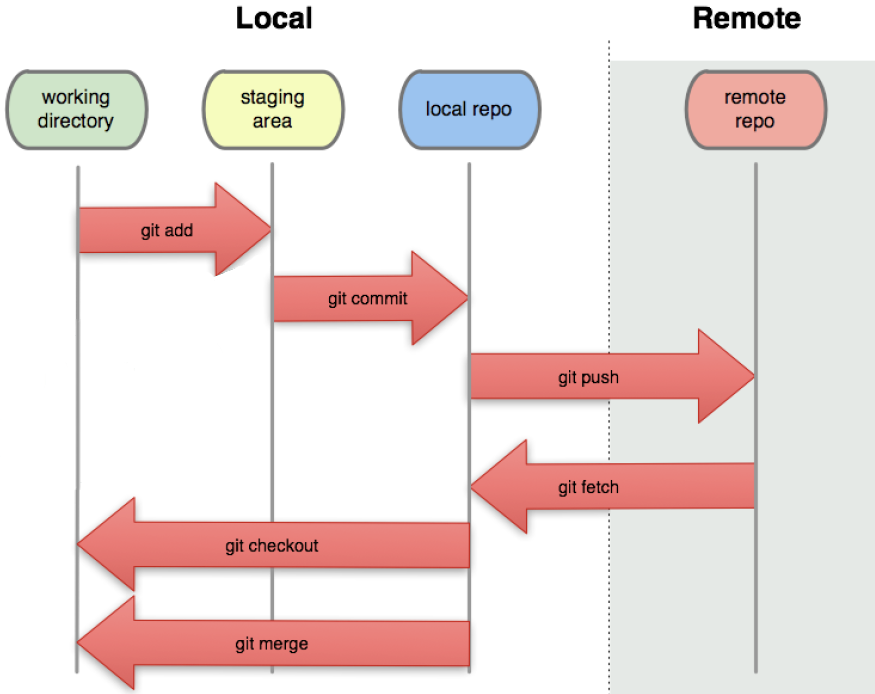
\includegraphics[width=0.57\textwidth]{../images/gitInteraktion.png}
		\end{center}
		
	\subsection{Unterschied: GIT und SVN}
		
		\begin{center}
			\begin{tabular}{c|c}
				\textbf{GIT}                                      & \textbf{SVN} \\
				\hline
				- Depot ist für jeden User \textbf{lokal}         & - Depot wird \textbf{auf einem Server} abgelegt \\
				- Operationen \textbf{offline ausführbar}         & - \textbf{Optimistisches Ausbuchen} \\
				- \textbf{Kryptografische Sicherung} der Historie & - Versioniert gesamtes Depot \\
				- Speichert \textbf{Schnappschüsse}               & - Speichert \textbf{Deltas} \\
			\end{tabular}
		\end{center}
		
	\subsection{Versionskontrolle}
		
		\subsubsection{Vorwärtsdelta}
		
			\textbf{Anfangsversion als Ausgangspunkt} und alle Deltas danach werden gespeichert.
			
		\subsubsection{Rückwärtsdelta}
			
			\textbf{Neueste Version als Ausgangspunkt} und alle Deltas davor werden gespeichert.
				
			\begin{tabular}{c|c|c}
				               & \textcolor{green}{\textbf{+}}      & \textcolor{red}{\textbf{-}} \\
				\hline
				Vorwärtsdelta  & Schneller Zugriff auf alte Version & Langsamer Zugriff auf neue Version \\
				\hline
				Rückwärtsdelta & Schneller Zugriff auf neue Version & Langsamer Zugriff auf alte Version \\
			\end{tabular}
			
		\subsubsection{Ein- und Ausbuchen}
		
			\begin{itemize}
				\item Optimistisch: \textbf{Mehrfaches} Ein- und Ausbuchen \textbf{ohne Änderungsreservierung}
				\item Strikt: Ein- und Ausbuchen \textbf{mit Änderungsreservierung}
			\end{itemize}